\documentclass[11pt,letterpaper,twoside]{report}

% System defined packages
\usepackage[hidelinks]{hyperref}
\usepackage{graphicx}
\usepackage{multicol}

% Custom defined packages
\usepackage{metrics}
\usepackage{fonts}
\usepackage{titlepage}
\usepackage{tableofcontents}
\usepackage{headers}
\usepackage{nicelistings}

\title{Using the Git Version Control System}
\author{Benjamin Woodruff}

\begin{document}
\maketitle
\maketoc

\chapter{Introduction}

A \strong{Version Control System (VCS)} helps a developer manage and
\emph{develop multiple revisions of source code, configuration files, or other
relevant documents}. Git is a modern VCS, with a fast distributed architecture.
It is open-source, and is open-source focused, originally developed to help
manage the development of the Linux Kernel, a multi-million line code base.

Git is implementation-transparent, and focuses on raw simplicity instead of
abstraction. It's underlying data storage and structures are stored as flat
files in the project directory. Deduplication is handled by linking.
Configuration is handled with plain text files, which can themselves be
versioned along with their project.

Compared to more traditional client-server architecture version control systems,
git is unique in that every developer owns an equal-value copy. This design
encourages forking by making the associated operation cheaper and easier. Git
advertises inexpensive branching and merging, which encourages developers to
separate changes, making later isolation of problems simpler.

This manual exists to provide the information necessary to become productive
with git, beginning with the basics and moving up. It assumes no knowledge,
except for a \emph{very basic understanding of the bash shell}. To avoid
verbosity, we assume git is already installed\footnote{For information on
installing git, refer to the official git documentation:
\url{http://git-scm.com/book/en/Getting-Started-Installing-Git}.}.

\vspace{\fill}
\begin{center}
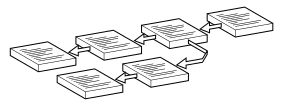
\includegraphics[height=5cm]{resources/branching_abstract.pdf}
\end{center}
\vspace*{\fill}

\chapter{Concepts}

Given that git itself is implementation transparent, and given that common
workflows that may arise from its use are quite different from a traditional
development process, it is imperative that one has a basic understanding of
git's design.

In git every state of the code is represented by an initial commit, and every
change after that\footnote{Don't worry: git caches intelligently, so that your
operations aren't O(\textit{n}) with respect to the commit chain length.}. What
that means is that every change is tracked discretely, and git knows
\emph{everything} about every stage of the development process.

\section{Branching}

Forming a branch \strong{breaks your development path in two}. That's a good
thing! We can make branches to add new features, fix bugs, or do anything else
we may want. Branching essentially allows us to context switch, and git tries to
make that process as smooth as possible.

One thing you'll hear often from the git community is that git has "cheap
branches". When git branches, instead of copying everything over, it simply
copies over the chain of commits that form the current branch, a fast operation.

\section{Merging}

When we're happy with our changes, we can merge things back, bringing our other
branch up-to-date.

Branching typically isn't difficult in version control systems, but merging
often is. Some systems have odd inconsistencies. The git competitor Subversion
performs linear merges, creating various edge cases that make merging complex,
or happen incorrectly. Git tracks previous merges and commits, reducing the
chance one of theses issues pops up. On top of that, it uses the industry-
standard 3-way merge algorithm, with inputs of the greatest common ancestor, the
existing branch, and the branch to merge into.

While you may not care how it works, rest assured: \emph{git's merging is some
of the best}.

\vspace{\fill}
\begin{flushright}

\includegraphics[width=9cm]{resources/patches_abstract.pdf}
\end{flushright}
\vspace*{\fill}

\chapter{Making a New Repository}

From an operating system's perspective, a git repository is just a directory.
There's nothing special running in the background, and the only marker is a
hidden subdirectory, '\texttt{.git}'. Let's turn a normal directory into a
repository with \cmdtt{git init}.

\begin{enumerate}
\item Open up your bash shell, or any other similar shell of your preference
\item If you already have a directory you would like to use (anything in it will
    be retained), navigate into to it with \cmdtt{cd}. If you don't, make a new
    directory with \cmdtt{mkdir}, and then \cmdtt{cd} into it
\item Run \cmdtt{git init}\footnote{All git commands are executed with
    \cmdtt{git} followed with a subcommand as an argument. To get a list of
    these subcommands, you can use \cmdtt{man git}. To look up documentation on
    a specific subcommand, replace the space with a dash. For example,
    \cmdtt{man git-init} will give you information on the init subcommand.} to
    initialize the repository
\end{enumerate}

\strong{Congratulations}, you've now made your first git repository! No data is
stored in git yet, however. If we want, we can verify this with
\cmdtt{ls .git}, showing us the contents of the \texttt{.git} directory we just
made:

\begin{multicols}{4}
\noindent
\texttt{branches/}\\
\texttt{config}\\
\texttt{description}\\
\texttt{HEAD}\\
\texttt{hooks/}\\
\texttt{info/}\\
\texttt{objects/}\\
\texttt{refs/}
\end{multicols}

We won't be playing directly with the contents of \texttt{.git} directly, but
it's good to know that it's there.

\section{Interesting Optional Arguments}

\begin{description}
\item[\texttt{--bare}]
    Running \cmdtt{git init --bare} will give you a special type of repository,
    known as a bare repository. Bare repositories have no checked out state, and
    so are generally not intended to be used directly. They are commonly used as
    a remote source, like on a server
\end{description}

\vspace{\fill}
\begin{flushright}

\includegraphics[height=3.5cm]{resources/new_stack_abstract.pdf}
\end{flushright}
\vspace*{\fill}

\chapter{Staging Changes}

After changes have been made, but before they're committed, they need to be
placed in the \strong{staging area}. The staging area \emph{lets you decide what
you do and don't want committed}. Examples of files you may not want
versioned include files generated by a compiler. \LaTeX{} generates lots of
extra files when building. When I compile this manual, for instance,
\cmdtt{latexmk} generates\footnote{\LaTeX{} is the document typesetting system
used to create this document. The additional files are logs, or other temporary
files used to speed up the next compilation.}:

\begin{multicols}{3}
\noindent
\texttt{manual.aux}\\
\texttt{manual.fdb\_latemk}\\
\texttt{manual.log}\\
\texttt{manual.out}\\
\texttt{manual.pdf}\\
\texttt{manual.toc}
\end{multicols}

I don't want to commit any of these files. With git, if I don't want them
committed, I simply won't stage them!

\section{Adding Changed Files to the Staging Area}
Let's assume we have both a file named \texttt{cake.py}, and a
directory\footnote{Git tracks only files, not directories. What this means is
that directories cannot be empty. If you want to stage or commit an empty
directory, you can put an empty \texttt{placeholder} file in the directory so
that git will see the folder.} called \texttt{src/} that we want to add. We can
use \cmdtt{git add} to accomplish this a variety of ways.

\vspace{.5em}\noindent
\strong{Adding the files sequentially is easy:}
\begin{enumerate}
\item Add the individual file with \cmdtt{git add cake.py}. The \texttt{add}
    subcommand takes the argument of the file to add.
\item Add the directory the same way you did the file, just passing the
    directory instead, with \cmdtt{git add src}
\end{enumerate}

\noindent
\strong{Grouping them is even easier:}
\begin{enumerate}
\item Add both the file and the directory by passing them both into the argument
    list with \cmdtt{git add cake.py src}
\item If you have a filename with spaces in it, you can group the character
    string in bash with single or double quotes:
    \cmdtt{git add "path with spaces.txt"}
\end{enumerate}

\noindent
\strong{If you want to commit all additions, it's even less work:}
\begin{enumerate}
\item Pass the current directory (represented by a period) with
    \cmdtt{git add .}
\item The \texttt{add} subcommand adds files recursively, so any new changes
    will be found and added for you
\end{enumerate}

% TODO: put something in here about git add --patch

\section{Staging file Removals}

While we haven't committed anything yet, if we had we could stage a file
removal.

\begin{enumerate}
\item Remove a file with \cmdtt{git rm}. If one wanted to remove
    \texttt{cake.py}, it would be as simple as running:
    
    \cmdtt{git rm cake.py}
\item To remove a directory, use the \texttt{rm} subcommand \emph{with the
    \texttt{-r} argument.} This is different from \cmdtt{git add}, which is
    recursive by default
\item By default, the subcommand both stages the removal, and deletes the file
    from the working directory if it exists. To only stage the removal, use
    \cmdtt{git rm --cached cake.py}
\item If you want to automatically add \emph{and remove} all the changed files,
    run \cmdtt{git add -u .} (without the \cmdtt{-u} argument,
    \cmdtt{git add}, git will only add files, not remove already deleted ones).
    Running this \emph{will not add files that aren't currently tracked by git}.
    That is to say it is not staged, nor has any state of the file been
    committed before
\end{enumerate}

\section{Checking the Staging Area Status}

Git can show you what changes are in the staging area, and which have been
changed but not staged with \cmdtt{git status}. It even shows helpful hints to
help you along!

For example, in repository where \texttt{cake.py} has been staged, but
\texttt{src/} has not yet:

\begin{lstlisting}[numbers=none]
# On branch master
#
# Initial commit
#
# Changes to be committed:
#   (use "git rm --cached <file>..." to unstage)
#
#       new file:   cake.py
#
# Untracked files:
#   (use "git add <file>..." to include in what will be committed)
#
#       src/
\end{lstlisting}

\vspace{\fill}
\begin{flushright}
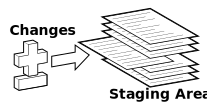
\includegraphics[height=4cm]{resources/staging_abstract.pdf}

\end{flushright}
\vspace*{\fill}

\chapter{Building a History with Commits}

While we've staged the changes, we haven't actually saved them yet. A commit can
be as \emph{small or large as you'd like}, but it should typically
\strong{accomplish one and only one thing} ("Fixes Bug \#56", "Restructures
\texttt{cake.py} API"). Git stores each commit as a diff (difference file) with
a message.

When you run \cmdtt{git commit}, it opens your default editor defined by the
bash \texttt{\$EDITOR} environment variable. You can override this behavior by
modifying the variable in your local \texttt{\textasciitilde/.bashrc} file or by
running

\cmdtt{git config --global core.editor vim}

replacing \texttt{vim}
with your editor of choice\footnote{Many GUI text editors will fork immediately,
tricking git into thinking that you exited with an unchanged commit file,
aborting the commit. You should consider using an command line editor like
\cmdtt{nano}, or you should look into arguments that can be passed into your
editor to keep it from forking.}.

\section{Making a Commit}

After changes have been made, running \cmdtt{git commit} with no extra arguments
will open your editor, giving it a commented file without any message:

\begin{lstlisting}[numbers=none]
# Please enter the commit message for your changes. Lines starting
# with '#' will be ignored, and an empty message aborts the commit.
# On branch master
#
# Initial commit
#
# Changes to be committed:
#   (use "git rm --cached <file>..." to unstage)
#
#   new file:   cake.py
#
# Untracked files:
#   (use "git add <file>..." to include in what will be committed)
#
#   src/
\end{lstlisting}

You can leave the comment block there, and simply \strong{put your commit
message above or below it}. A properly formatted commit message should:

\begin{itemize}
\item Begin with a capitalized 50 (or less) character title. This is used when
    git needs to display a short description, so it should stand on its own
\item Include a general description of what the commit adds in a paragraph below
    the one-line description, separated by an empty line. More paragraphs may
    follow (each separated from each other by a blank line), and bulleted lists
    are acceptable
\item Should be wrapped to 72 characters, just like one would do with source
    code, or on a typewriter
\item Be written in present tense. Say "Adds new feature", rather than "Added
    new feature". Say what it \emph{does}, not what it \emph{did}
\end{itemize}

As an example, here is a well-formatted commit message:

% TODO: Cite http://tbaggery.com/2008/04/19/a-note-about-git-commit-messages

\begin{lstlisting}[numbers=none]
Adds cake.py to compute cake radii

By dividing the circumference by 2pi, we get a radius. The
to_radius(circ) function performs the calculation in an efficient manor.

The function is:

- Fast

- Really, really, awesome. It will be used to restructure the rest of the
  mathematical code
\end{lstlisting}

\section{Interesting Optional Arguments}

\begin{description}
\item[\texttt{-a}, \texttt{--all}]
    \cmdtt{git commit -a} is equivalent to running \cmdtt{git add -u .} followed
    by \cmdtt{git commit}
\item[\texttt{--interactive}]
    Running \cmdtt{git commit --interactive} allows you to interactively pick
    what files to add or remove before committing. This can also be used as
    \cmdtt{git add --interactive}, but it tends to be more useful with the
    \texttt{commit} subcommand
\item[\texttt{-m}, \texttt{--message}]
    You can write a simple one-line commit message without opening a text editor
    by running \cmdtt{git commit -m "Adds cake.py to compute cake radii"}. This
    argument is useful, but should usually be avoided in favor of a longer, more
    descriptive commit message
\end{description}

\section{The Commit Log}

Running \cmdtt{git log} will show you a history of all your previous commits in
reverse-chronological order. The output is paged with \cmdtt{less}, making it
easily scrollable and searchable. If you'd like a more compressed output, you
can use the \texttt{--oneline} argument, which will show the one-line summary of
each commit instead of a full summary.

You'll notice that each commit is assigned a 40-character alphanumeric
hexadecimal string. This is a cryptographic hash used both to ensure data
integrity, and to \emph{identify commits}. When referencing commits yourself,
you only need to use the first few characters of the hash, and git can figure
out the rest.

%\vspace{\fill}
%\begin{center}
%
\includegraphics[height=5cm]{resources/timeline_abstract.pdf}
%\end{center}
%\vspace*{\fill}

\chapter{Branching Out}

Software rarely follows a linear path. It's not something you write from
beginning to end, nor something you typically revise incrementally. Multiple
developers may want to work on different parts at the same time, but they should
also be able to easily see how their changes affect others. Perhaps one of the
most useful features of a VCS, and especially a distributed VCS like git, is the
ability to develop multiple versions in parallel. You can do this with multiple
forks, but with branches, you can do it in a more centralized, orderly, and
minimal manor.

\section{The "master" Branch}

If you run \cmdtt{git branch} without any arguments (assuming you've committed
something first) you'll see

\begin{lstlisting}[numbers=none]
* master
\end{lstlisting}

\cmdtt{git branch} lists all local branches in the repository, and puts an
asterisk next to the active one. What this is saying is that we have one branch,
named master, and it is currently checked out (active).

When there's not any branches, git silently creates one for you. Many projects
use the master branch as their primary branch, or as their release branch, but
you're under no obligation to use it. You can make a new branch and delete
\texttt{master} if you want, it's up to you. Regardless, it's our starting
point.

\section{Forming a Branch}

Making a new branch is as simple as calling \cmdtt{git branch} with an name
argument. Specifying a branch to start from can be done by passing two
arguments. To form a new branch with \texttt{master} as our starting point, we
could call \cmdtt{git branch new-branch-name} while \texttt{master} is checked
out, or \cmdtt{git branch master new-branch-name} to work from \texttt{master}
explicitly, regardless of the currently checked out branch.

People tend to like to group their branches like when making feature
branches\footnote{Temporary branches for adding a new experimental feature}. A
common way of doing this is to use forward slashes like directory names, for
example, \texttt{feature/some-feature-name}. Git handles these special branch
names internally by actually creating a separate subdirectory in \texttt{.git}.

\section{Switching to a Branch}

Suppose you've made a new branch named \texttt{feature/pie}, which you're going
to use to try to add pie support in addition to your preexisting cake support.
You run \cmdtt{git branch}, and to your surprise, you see

\begin{lstlisting}[numbers=none]
  feature/pie
* master
\end{lstlisting}

The asterisk is still by master! To activate the new branch, we need to use
\cmdtt{git checkout}. The subcommand clears the working directory (don't worry,
git is still keeping track of it), replacing it with the last state of a given
branch, or to the state of a given branch. Simply pass \cmdtt{git checkout} a
branch name or the first few characters of a commit hash\footnote{Commit hashes
can be found by running \cmdtt{git log}.}, and git will either jump to the
alternate reality, or shoot you back in time\footnote{If you decide to play with
going back in time, be careful not to change anything without branching first.
Like in the plot of many science fiction movies, bad things could happen.}.

\vspace{\fill}
\begin{center}

\includegraphics[height=5cm]{resources/example_branching.pdf}
\end{center}
\vspace*{\fill}

\chapter{Going Forward}

Git is an incredible tool with over 150 subcommands as of writing, each with
their own different arguments and options. Beyond just subcommands, git has many
different uses and workflows. Git isn't limited to just code either. People
store their configuration files in it. Developers store documentation alongside
their code in git. Even this document is backed by git.

There are different 3rd-party projects built on top of git, like
\cmdtt{git-flow}, \cmdtt{git-annex}, and \cmdtt{git-media}. Some of them help
with everyday git usage, others enable you to do things with git you'd never
imagine.

The goal of this manual was to spark you interest, and to push you over the
initial bumps in the learning curve. The rest of the climb is yours, and I hope
you enjoy it. I'll see you at the top!

\section{Sources of Documentation}

\begin{description}
\item[\href{http://git-scm.com/documentation}{git-scm.com}]
    The official git website has a plethora of documentation, including free
    access to the popular e-book, "Pro Git"
\item[Man Pages]
    We've mentioned it before, but you can look up documentation on (almost) any
    git subcommand by replacing the space with a hyphen, and passing it to man.
    For instance: \cmdtt{man git-add}. If you prefer, you can alternatively use
    the help subcommand: \cmdtt{git help add}
\item[\href{http://www-cs-students.stanford.edu/~blynn/gitmagic/}{git-magic}]
    Available for free from
    \url{http://www-cs-students.stanford.edu/~blynn/gitmagic/}, git-magic goes
    into great depth on everything from the same basics covered in this manual
    to the underlying flaws of git and the internal organization of git's secret
    \texttt{.git} directory
\end{description}

\vspace{\fill}
\begin{flushright}
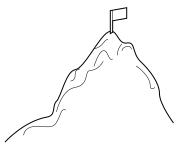
\includegraphics[height=6cm]{resources/learning_curve_abstract.pdf}
\end{flushright}
\vspace*{\fill}

\end{document}
